\section{Results}
\label{sec:results}

\subsection{Main Comparison: LoRA Achieves Best Balanced Performance}
\label{sec:main}

Table~\ref{tab:main} summarizes continual learning results (n\_shot=32, seeds 42--44). \textbf{Sequential FT} suffers catastrophic forgetting: T1 Dice drops from 0.80 to 0.16 after T2 (BWT$\approx$-0.65). \textbf{Sequential Linear} achieves strong T1 (0.79) with mild forgetting, but fails on T2 (MAE 1.45). \textbf{EWC} achieves strong T1 Dice (0.79) and very low T2 MAE (0.001); T1 after T2 shows high variance (0.15$\pm$0.24) with BWT$\approx$-0.65. \textbf{LwF} and \textbf{Replay} achieve strong T1 Dice ($\sim$0.79--0.80) and low T2 MAE (0.020--0.021); LwF T1 after T2=0.25$\pm$0.22 (BWT$\approx$-0.56); Replay T1 after T2=0.01$\pm$0.01 (BWT$\approx$-0.78). \textbf{LoRA} attains competitive T1 Dice (0.60) with the best T2 MAE (0.012) among continual methods, and BWT=0. Paired $t$-tests across seeds (n=3): LoRA vs.\ Sequential Linear on T2 MAE is highly significant (LoRA better, $p=0.001$); on T1 Dice, Sequential Linear is higher (bootstrap 95\% CI for difference: [0.08, 0.27], $p=0.09$).

\begin{table}[t]
\caption{Main continual learning results (mean$\pm$std over seeds 42--44, n\_shot=32). BWT negative = forgetting. $^\dagger$Seq FT and EWC T2 MAE likely overfit on few-shot validation (MAE $<$0.01 implausible; per-task linear achieves 0.063 on full eval).}
\label{tab:main}
\centering
\begin{tabular}{lcccc}
\toprule
Method & T1 Dice$\uparrow$ & T2 MAE$\downarrow$ & T1 after T2 & BWT \\
\midrule
LoRA (enc+dec) & $0.60 \pm 0.08$ & $0.012 \pm 0.003$ & (=T1) & $\mathbf{0.00}$ \\
Sequential Linear & $0.79 \pm 0.01$ & $1.45 \pm 0.03$ & $0.78 \pm 0.01$ & $-0.01 \pm 0.01$ \\
Sequential FT & $0.80 \pm 0.02$ & $0.005^\dagger \pm 0.003$ & $0.16 \pm 0.19$ & $-0.65 \pm 0.17$ \\
EWC & $0.79 \pm 0.02$ & $0.001^\dagger \pm 0.001$ & $0.15 \pm 0.24$ & $-0.65 \pm 0.23$ \\
LwF & $0.80 \pm 0.02$ & $0.020 \pm 0.009$ & $0.25 \pm 0.22$ & $-0.56 \pm 0.24$ \\
Replay & $0.79 \pm 0.01$ & $0.021 \pm 0.013$ & $0.01 \pm 0.01$ & $-0.78 \pm 0.02$ \\
\bottomrule
\end{tabular}
\end{table}

Table~\ref{tab:extended} extends the comparison with per-task linear probing (separate model per task, no continual; patch=32, epochs=50, differing from continual scripts). Per-task linear achieves T2 MAE 0.063 on full eval, which serves as a sanity check: EWC (0.001) and Sequential FT (0.005) are implausibly low and likely overfit on few-shot validation. LwF and Replay achieve strong T1 Dice and low T2 MAE (0.020--0.021); LoRA offers competitive T2 MAE (0.012) with zero forgetting.

Figure~\ref{fig:task1} and~\ref{fig:task2} show representative qualitative results (see Appendix for full six-sample stacks). Common LoRA failure modes---e.g., under-segmentation of tumor boundaries and systematic age underestimation---are documented in the Appendix (Fig.~\ref{fig:app_seg_failure},~\ref{fig:app_age_failure}). On the IXI validation set (n=109, seed 42), a paired Wilcoxon signed-rank test on prediction residuals indicated significant systematic bias ($p<0.001$): the model tends to underestimate brain age. \textbf{IXI age label caveat:} IXI subjects with missing age in the metadata are imputed to 50.0\,yr in our preprocessing; the six ``best'' samples in Fig.~\ref{fig:app_age_stack} (lowest prediction error) all have ground-truth 50.0\,yr, suggesting a concentration of imputed labels. This limits the interpretability of T2 MAE on validation; we report it transparently.

\begin{figure}[t]
\centering
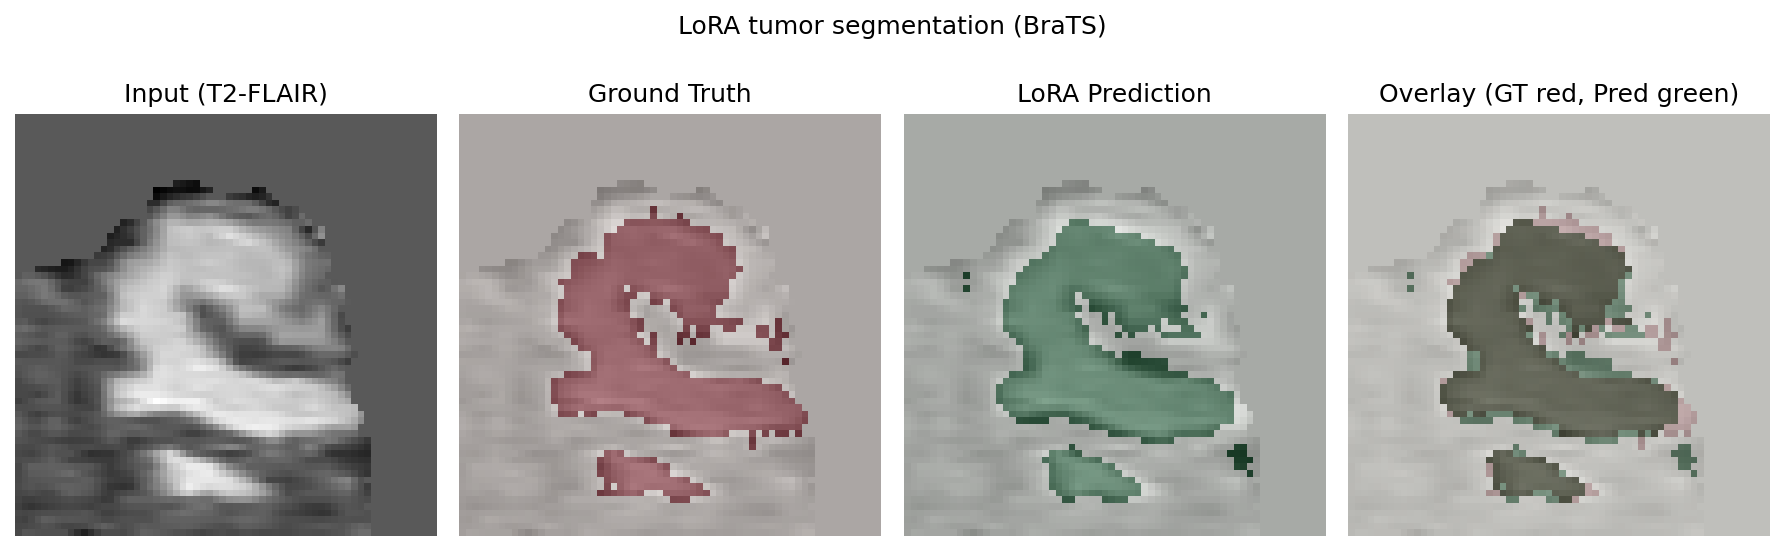
\includegraphics[width=0.7\textwidth]{figures/show_case_task2.png}
\caption{Task 1 tumor segmentation (BraTS): representative sample. Input (T2-FLAIR), Ground Truth, LoRA prediction, overlay (red=GT, green=pred). Full six-sample figure in Appendix (Fig.~\ref{fig:app_seg_stack}).}
\label{fig:task1}
\end{figure}

\begin{figure}[t]
\centering
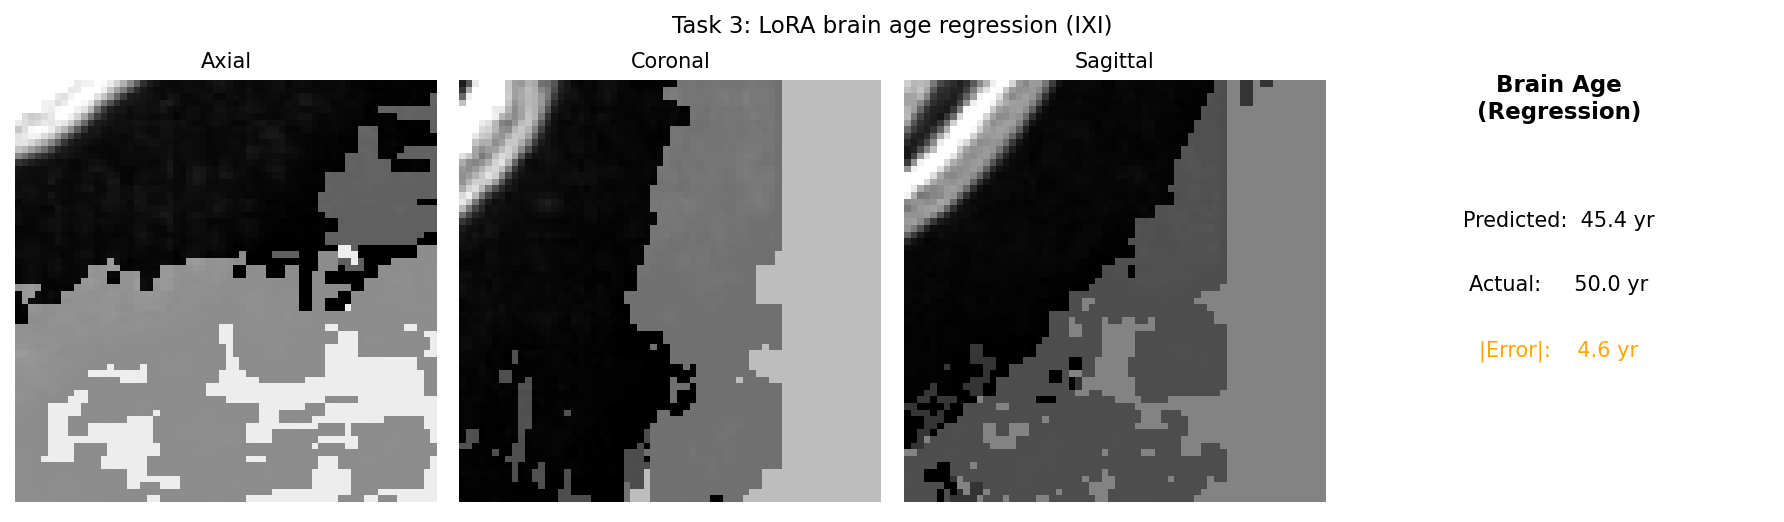
\includegraphics[width=0.7\textwidth]{figures/task3_age_s42_0.png}
\caption{Task 2 brain age regression (IXI): representative sample. Orthogonal MRI views (Axial, Coronal, Sagittal) and predicted vs.\ actual age. Full six-sample figure in Appendix (Fig.~\ref{fig:app_age_stack}).}
\label{fig:task2}
\end{figure}

\begin{table}[t]
\caption{Extended comparison. Per-task: separate model per task (patch=32, epochs=50; not continual). EWC and Seq FT T2 MAE likely overfit (see Table~\ref{tab:main}).}
\label{tab:extended}
\centering
\begin{tabular}{lcccl}
\toprule
Method & T1 Dice$\uparrow$ & T2 MAE$\downarrow$ & Setting \\
\midrule
LoRA (enc+dec) & $0.60 \pm 0.08$ & $\mathbf{0.012} \pm 0.003$ & Continual \\
EWC & $0.79 \pm 0.02$ & $0.001^\dagger \pm 0.001$ & Continual \\
LwF & $0.80 \pm 0.02$ & $0.020 \pm 0.009$ & Continual \\
Replay & $0.79 \pm 0.01$ & $0.021 \pm 0.013$ & Continual \\
Sequential Linear & $0.79 \pm 0.01$ & $1.45 \pm 0.03$ & Continual \\
Sequential FT & $0.80 \pm 0.02$ & $0.005^\dagger \pm 0.003$ & Continual (forgets) \\
Per-task Linear & 0.65 & 0.063 & Oracle (no continual) \\
\bottomrule
\end{tabular}
\end{table}

\subsection{Catastrophic Forgetting in Sequential FT}
\label{sec:forgetting}

Sequential FT achieves high T1 Dice (0.80) and very low T2 MAE (0.005) immediately after training each task. The latter likely reflects overfitting on few-shot validation. Crucially, T1 Dice after T2 training collapses to 0.16 (mean over seeds), yielding $\Delta \approx 0.64$---a clear demonstration of catastrophic forgetting when the backbone is overwritten for T2.

\subsection{LoRA Ablation: Encoder-only vs Encoder+Decoder}
\label{sec:lora_ablation}

Table~\ref{tab:lora_ablation} compares LoRA placement. Encoder-only LoRA yields poor T1 Dice (0.19); encoder+decoder yields 0.50. Decoder adaptation is necessary for segmentation. T2 (regression) is similar for both.

\begin{table}[t]
\caption{LoRA placement ablation. Enc+dec = encoder+decoder.}
\label{tab:lora_ablation}
\centering
\begin{tabular}{lcc}
\toprule
LoRA Config & T1 Dice$\uparrow$ & T2 MAE$\downarrow$ \\
\midrule
Encoder-only & 0.19 & 0.20 \\
Encoder+decoder & \textbf{0.50} & 0.20 \\
\bottomrule
\end{tabular}
\end{table}

\subsection{Shot Ablation (n\_shot=16 vs 32 vs 64)}
\label{sec:shot}

Table~\ref{tab:shot} shows few-shot sensitivity for LoRA. At n\_shot=16, LoRA attains T1 Dice 0.45$\pm$0.04 and T2 MAE 0.33$\pm$0.01; n\_shot=32 improves both (T1 0.62, T2 MAE 0.16). Fewer shots degrade performance, especially for segmentation.

Table~\ref{tab:shot64} reports n\_shot=64 results for EWC and LwF. EWC attains higher T1 Dice (0.84$\pm$0.02) than at n\_shot=32 (0.79) but T2 MAE remains implausibly low (0.001$^\dagger$) and BWT$\approx$-0.77. LwF at n64: T1 Dice 0.82$\pm$0.01, T2 MAE 0.038$\pm$0.014; T1 after T2 shows high variance (0.25$\pm$0.41).

\begin{table}[t]
\caption{Shot count ablation (LoRA enc+dec, seeds 42--43 for n\_shot=16).}
\label{tab:shot}
\centering
\begin{tabular}{lcc}
\toprule
n\_shot & T1 Dice$\uparrow$ & T2 MAE$\downarrow$ \\
\midrule
16 & $0.45 \pm 0.04$ & $0.33 \pm 0.01$ \\
32 & $0.62 \pm 0.07$ & $0.16 \pm 0.05$ \\
\bottomrule
\end{tabular}
\end{table}

\begin{table}[t]
\caption{n\_shot=64 results (EWC, LwF; seeds 42--44). $^\dagger$EWC T2 MAE likely overfits.}
\label{tab:shot64}
\centering
\begin{tabular}{lcccc}
\toprule
Method & T1 Dice$\uparrow$ & T2 MAE$\downarrow$ & T1 after T2 & BWT \\
\midrule
EWC & $0.84 \pm 0.02$ & $0.001^\dagger \pm 0.0003$ & $0.07 \pm 0.10$ & $-0.77 \pm 0.11$ \\
LwF & $0.82 \pm 0.01$ & $0.038 \pm 0.014$ & $0.25 \pm 0.41$ & $-0.58 \pm 0.42$ \\
\bottomrule
\end{tabular}
\end{table}

\subsection{Phase 3 (t32\_t3t2: Task Order T3$\to$T2)}
\label{sec:t32}

Table~\ref{tab:t32} reports Phase 3 results with \textbf{task order T3$\to$T2} (regression first, then segmentation; seeds 42--44). BWT measures T3 forgetting: T2 MAE after T1 training minus T2 MAE right after T2; positive = forgetting. LoRA attains T1 Dice 0.50$\pm$0.08 and T2 MAE 0.005$\pm$0.002 with BWT=0. Sequential Linear: T1 0.78$\pm$0.01, T2 MAE 0.26$\pm$0.003; T2 after T1 = 0.36$\pm$0.05 (BWT$\approx$0.10). Sequential FT: T2 MAE 0.001$^\dagger$ right after T2, but collapses to 7.17$\pm$1.41 after T1 training (BWT$\approx$7.16)---severe catastrophic forgetting of regression when the backbone is overwritten for segmentation.

\begin{table}[t]
\caption{Phase 3 (t32\_t3t2, T3$\to$T2 order, n\_shot=32). BWT = T2 MAE after T1 minus T2 MAE after T2 (positive = T3 forgetting). $^\dagger$Seq FT T2 MAE likely overfits.}
\label{tab:t32}
\centering
\begin{tabular}{lcccc}
\toprule
Method & T1 Dice$\uparrow$ & T2 MAE$\downarrow$ & T2 after T1 & BWT \\
\midrule
LoRA (enc+dec) & $0.50 \pm 0.08$ & $0.005 \pm 0.002$ & --- & $\mathbf{0.00}$ \\
Sequential Linear & $0.78 \pm 0.01$ & $0.26 \pm 0.003$ & $0.36 \pm 0.05$ & $0.10 \pm 0.05$ \\
Sequential FT & $0.81 \pm 0.01$ & $0.001^\dagger \pm 0.0003$ & $7.17 \pm 1.41$ & $7.16 \pm 1.41$ \\
\bottomrule
\end{tabular}
\end{table}

\subsection{Per-Seed Breakdown (LoRA, n\_shot=32)}
\label{sec:per_seed}

Table~\ref{tab:per_seed} reports per-seed LoRA results for reproducibility. T1 Dice ranges 0.52--0.68; T2 MAE 0.008--0.014.

\begin{table}[t]
\caption{Per-seed LoRA results (enc+dec, n\_shot=32).}
\label{tab:per_seed}
\centering
\begin{tabular}{lcc}
\toprule
Seed & T1 Dice$\uparrow$ & T2 MAE$\downarrow$ \\
\midrule
42 & 0.523 & 0.014 \\
43 & 0.598 & 0.008 \\
44 & 0.680 & 0.012 \\
\bottomrule
\end{tabular}
\end{table}

\subsection{Resource Usage}
\label{sec:resource}

Table~\ref{tab:resource} summarizes compute. LoRA adds $<$0.1\% trainable params per task; T1 (segmentation) uses $\sim$1.7\,GB peak GPU.

\begin{table}[t]
\caption{Resource usage (LoRA, n\_shot=32).}
\label{tab:resource}
\centering
\begin{tabular}{lccc}
\toprule
Task & Params (trainable) & GPU peak (MB) & Time (sec) \\
\midrule
T1 (segmentation) & 46,872 & 1,670 & $\sim$4k--26k \\
T2 (regression) & 28,177 & 688 & $\sim$95--780 \\
\bottomrule
\end{tabular}
\end{table}
